%%******************************************************************************
%%
%% introduction.tex
%%
%%******************************************************************************
%%
%% Title......: Introduction
%%
%% Author.....: GSCAR-DFKI
%%
%% Started....: Nov 2013
%%
%% Emails.....: renan028@gmail.com
%%
%% Address....: Universidade Federal do Rio de Janeiro
%%              Caixa Postal 68.504, CEP: 21.945-970
%%              Rio de Janeiro, RJ - Brasil.
%%
%%******************************************************************************


%%******************************************************************************
%% SECTION - Eletronica
%%******************************************************************************

\section{Propostas de soluções para a arquitetura da eletrônica do Projeto ROSA}

Foram desenvolvidas três soluções para a arquitetura da eletrônica, que podem ser classificadas quanto à simplicidade, custo e rapidez de execução.

A primeira solução consiste em projetar uma placa que pudesse realizar o
controle da alimentação dos dispositivos da eletrônica, monitoramento elétrico
de corrente e voltagem, e gerenciar os dispositivos, com todas as interfaces de
comunicação do sistema. O processamento do sonar será realizado por um PC na
base. Os componentes da eletrônica necessários para a proposta são de baixo
custo, porém há complexidade de software e eletrônica em relação às outras soluções, o que impacta em uma maior demora da solução.

A segunda proposta incide na utilização de um PC embarcado para o processamento
de sinal e gerenciamento de todas as interfaces necessárias para o
gerenciamento dos dispositivos. O PC embarcado se comunica com a base por
Ethernet, onde haverá um roteador para estabelecer a comunicação com o Tablet.
Esta solução necessita de um PC104 embarcado, com proteção mecânica desenvolvida
pela equipe, ou uma eletrônica importada protegida. Do ponto de
vista da eletrônica, a solução tem com PC104 apresenta custo intermediário, é
simples e de baixo tempo de execução, porém há a complexidade mecânica. Por
outro lado, a eletrônica importada é de alto custo, mas aproxima-se mais de um
produto final. 

A terceira proposta é a utilização de dois PCs, de forma que haja
processamento tanto na eletrônica embarcada, quanto na base. O custo desta solução é alto, porém apresenta grande simplicidade e rápido tempo de execução.

\section{Proposta 1 – Placa com Microcontrolador e Gateway Ethernet}

A eletrônia é composta pelos seguintes dispositivos:
\begin{itemize}
  \item Dois Encoders da IFM: 24V e interface CAN. Datasheet em Anexo 1.
  \item Um sonar Super SeaKing da Tritech: 24V e interface RS232. Datasheet em
  Anexo 1
  \item Um Sistema Pan \& Tilt da Kongsberg: 24V e interface RS485. Datasheet em
  Anexo 1.
  \item Dois sensores Indutivos da Pepperl-Fuchs: 24V e saída analógico.
  Datasheet em Anexo 1.
  \item Um sensor de inclinação da Pepperl-Fuchs: 24V e saída analógica.
  Datasheet em Anexo 1.
  \item Um sensor de pressão da Velki: 24V e saída RS485. Datasheet em Anexo 1.
\end{itemize}	

A placa com microcontrolador deve ter disponível todas as alimentações elétricas
e interfaces de comunicação descritas acima, além de saída Ethernet para
comunicação com a base. Na figura~\ref{placa}, pode ser observado o modelo 3D da
placa. Na figura~\ref{alimentacao_placa} e figura~\ref{com_placa}, são
representados os diagramas de interfaces de comunicação e alimentação elétrica, respectivamente, do sistema. A seguir, será feita uma breve explicação dos principais componentes da placa.

O microcontrolador AT90CAN64 será responsável pelo monitoramento e controle da alimentação elétrica de todos os dispositivos, além de ser o responsável pela comunicação CAN com o Encoder. 

O gateway Ethernet SR01E12 possui interfaces UART e analógicas. Dessa forma, diversos dispositivos podem se conectar ao gateway através de chips MAX232 ou MAX485, que realizam a conversão RS232 ou RS485 para UART, respectivamente.
  
\begin{figure}[H]
    \centering
    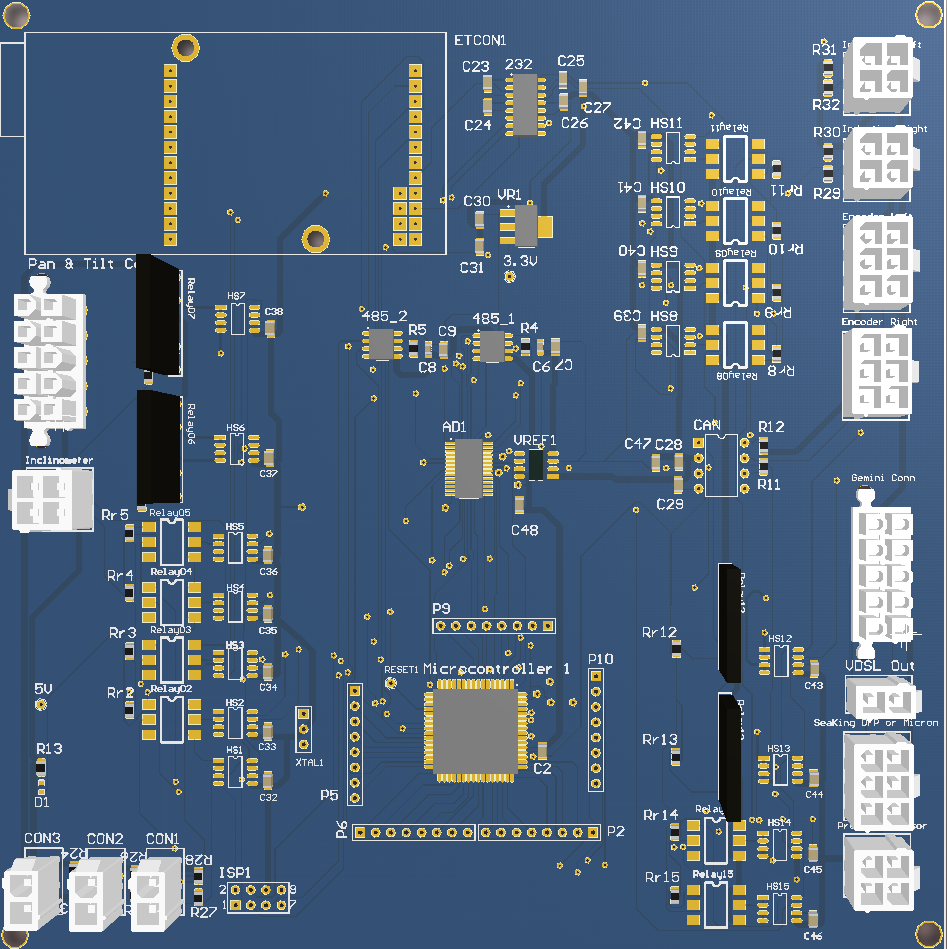
\includegraphics[width=1\columnwidth]{figs/eletronica/1.png}
    \caption{Placa 3D}
    \label{placa}
\end{figure}

\begin{figure}[H]
    \centering
    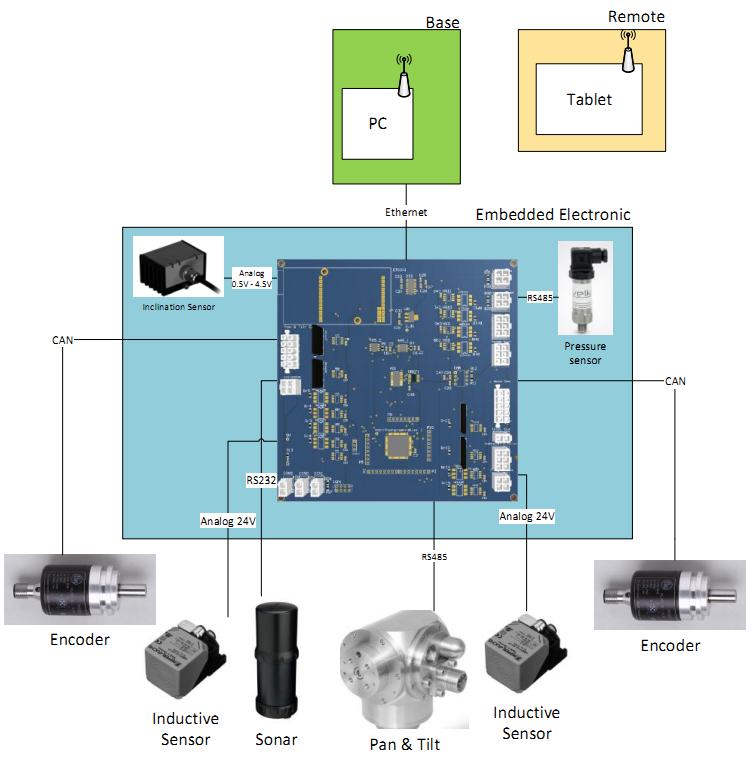
\includegraphics[width=1\columnwidth]{figs/eletronica/2.png}
    \caption{Diagrama de Alimentações}
    \label{alimentacao_placa}
\end{figure}

\begin{figure}[H]
    \centering
    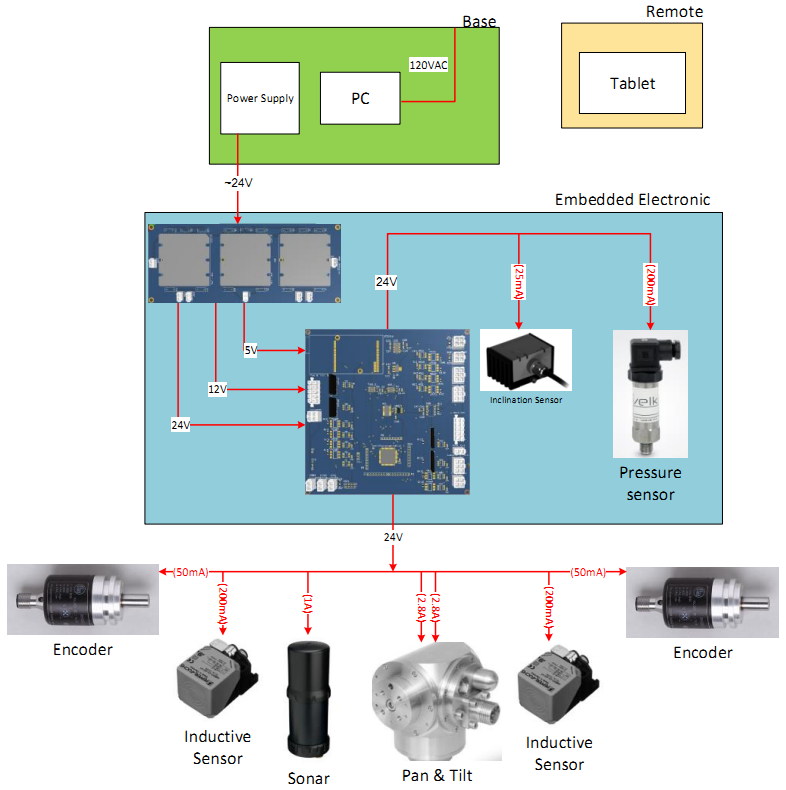
\includegraphics[width=1\columnwidth]{figs/eletronica/3.png}
    \caption{Diagrama de Comunicação}
    \label{com_placa}
\end{figure}
 
A placa com microcontrolador é uma solução de baixo custo, porém exige maior tempo de execução. Há a necessidade de fabricação, montagem, testes elétricos e lógicos da placa e programação de microcontrolador para gerenciamento de cada interface, como o protocolo CANOpen. 
A eletrônica deverá ser acoplada ao Lifting Beam, logo deverá ser construída uma estrutura mecânica à prova d’água para esta solução.


\section{Proposta 2 – PC Embarcado e base com Roteador}

A solução com um PC embarcado, acoplado à estrutura do Lifting Beam, é
considerada uma solução intermediária em relação ao custo e é uma solução que
mais se aproxima ao produto final. Esta solução é menos suscetível a falhas
elétricas e de gerenciamento de dispositivos, quando comparada com a solução da
placa com microcontrolador. Além disso, o tempo de execução gasto para programação de microcontrolador e fabricação da placa justifica a aquisição de um PC104. Na figura~\ref{pc104}, podemos observar o diagrama de interfaces desta solução.

\begin{figure}[H]
    \centering
    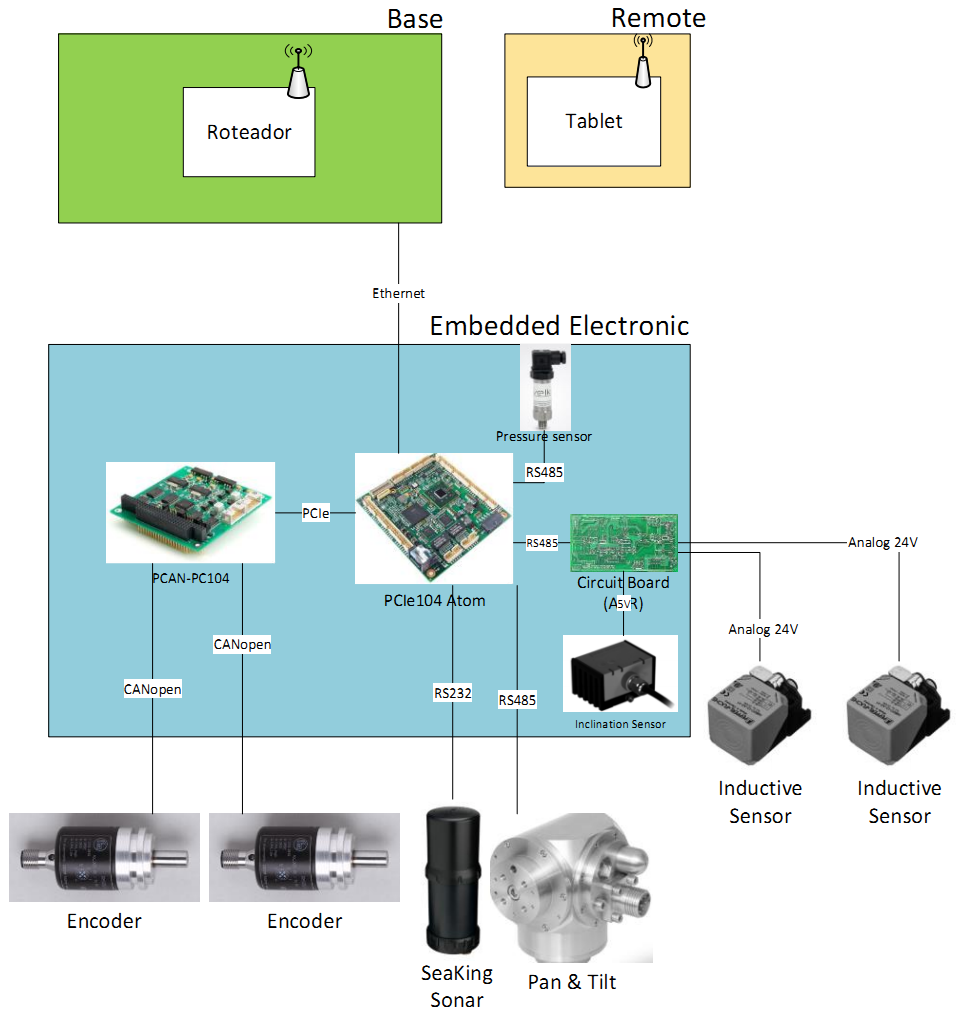
\includegraphics[width=1\columnwidth]{figs/eletronica/4.png}
    \caption{Diagrama de Comunicações - PC104}
    \label{pc104}
\end{figure} 
 
Assim como a solução 1, deverá ser construída uma estrutura mecânica à prova d’água.

\section{Proposta 3 – PC embarcado e PC na base}

A terceira solução consiste em realizar tanto um processamento na eletrônica
embarcada, quanto na base. Poderá ser utilizado tanto uma eletrônica importada
com Pelican Case quanto uma solução semelhante a 2, com PC104, e um laptop a
base. Observar a figura~\ref{prop3}.

\begin{figure}[H]
    \centering
    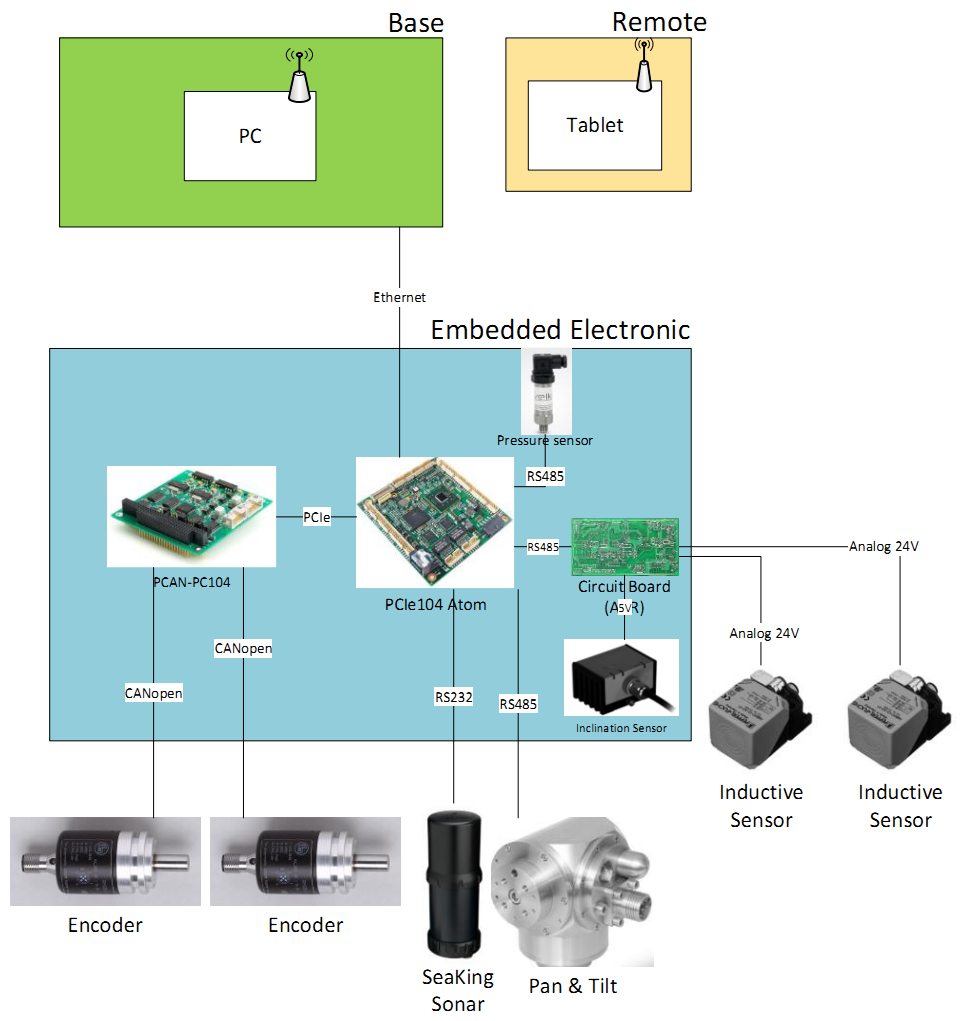
\includegraphics[width=1\columnwidth]{figs/eletronica/5.png}
    \caption{Diagrama de Comunicações - Proposta 3}
    \label{prop3}
\end{figure} 

\section{Estágio atual do projeto}

Concluído:
\begin{itemize}
  \item Projeto conceitual;
  \item Pesquisa, compra e recebimento de sensores Indutivos;
  \item Pesquisa, compra e recebimento de encoders;
  \item Pesquisa e compra de Sonar (importação);
  \item Pesquisa e compra de sistema Pan \& Tilt (importação);
  \item Pesquisa e compra de sensor de Pressão;
  \item Teste com sensores indutivos;
  \item Pesquisa, compra e recebimento de Tablet;
  \item Projetos de placas com microcontrolador;
  \item Projeto de placa com conversores para alimentação elétrica;
  \item Pesquisa de PC104 e acessórios;   
\end{itemize}
Em andamento:
\begin{itemize}
  \item Aplicativo para interface do sistema com usuário.
  \item Compra de PC104 e acessórios para a solução 2.
  \item Revisão da placa.
  \item Set-up para teste de bancada com sonar.
\end{itemize}